% Generated by resultspart1.py
% Preamble: \usepackage{graphicx,booktabs}
%           \graphicspath{{results_part1/figures/}}
% Move the blocks around freely; each is self-contained.

% ======================================================================
% Set-up
% ======================================================================
% Generated by resultspart1.py -- do not edit by hand
\begin{table}[!t]
\centering
\caption{Simulation set-up. All runs use forward Euler with $h=0.05$\,s, ideal thrusters (Part 1 default), start at $\eta_0=[0,0,0]^\top$, $\nu_0=0$, and the same controller and thrust allocation.}
\label{tab:sim_setup}
\footnotesize
\setlength{\tabcolsep}{3pt}
% shrink-to-fit: scaled down only if wider than the column/page
\sbox0{%
\begin{tabular}{lllcc}
\toprule
Sim. & Setpoint & Environment & Ref. & $T$ [s] \\
\midrule
1a & $[0,0,0]^\top$ & Current $0.5$\,m/s from east & On & $800$ \\
1b & $[0,0,0]^\top$ & Wind $15$\,m/s from east, $\sigma=1$\,m/s & On & $800$ \\
2 & $[0,0,0]^\top$ & Current $0.5$\,m/s, N$\to$E in 300\,s & On & $900$ \\
3 & $[10,10,3\pi/2]^\top$ & None & On / Off & $600$ \\
4 & Four corners & None & On & $1500$ \\
\bottomrule
\end{tabular}}
\ifdim\wd0>\linewidth\resizebox{\linewidth}{!}{\usebox0}\else\usebox0\fi
\end{table}


% ======================================================================
% Simulation 1: station keeping
% ======================================================================
% Generated by resultspart1.py -- do not edit by hand
\begin{table}[!t]
\centering
\caption{Simulation 1: station-keeping performance at $\eta_{sp}=[0,0,0]^\top$. SS = steady state (mean over the last 100\,s of the 800\,s run). TB = Tunnel Bow, A1/A2 = Azimuth 1/2.}
\label{tab:sim1}
\footnotesize
\setlength{\tabcolsep}{3pt}
% shrink-to-fit: scaled down only if wider than the column/page
\sbox0{%
\begin{tabular}{lcc}
\toprule
Metric & 1a: current & 1b: wind \\
\midrule
Max.\ position error [m] & $1.12$ & $1.60$ \\
\quad at time [s] & $35$ & $32$ \\
Max.\ $|e_N|$ / $|e_E|$ [m] & $0.00$ / $1.12$ & $0.05$ / $1.60$ \\
Max.\ heading error [deg] & $0.09$ & $2.04$ \\
Settling, pos.\ ($<0.5$\,m) [s] & $82.1$ & $88.5$ \\
Settling, head.\ ($<1^\circ$) [s] & $0.0$ & $72.4$ \\
\midrule
SS mean position error [m] & $0.000$ & $0.177$ \\
SS RMS position error [m] & $0.000$ & $0.207$ \\
SS mean heading error [deg] & $0.000$ & $0.207$ \\
SS thr.\ $X$/$Y$/$N_z$ [kN, kNm] & $0.0$/$17.0$/$0.0$ & $0.0$/$27.9$/$55.2$ \\
SS wind $X$/$Y$/$N_z$ [kN, kNm] & -- & $0.0$/$-27.8$/$-55.1$ \\
\midrule
SS mean thrust TB/A1/A2 [kN] & $8.7$/$4.2$/$4.2$ & $16.4$/$5.9$/$5.9$ \\
Peak thrust TB/A1/A2 [kN] & $9.2$/$4.5$/$4.5$ & $18.9$/$6.8$/$6.8$ \\
Peak util.\ TB/A1/A2 [\%] & $29$/$6$/$6$ & $59$/$9$/$8$ \\
Time saturated [\%] & $0.0$ & $0.0$ \\
\bottomrule
\end{tabular}}
\ifdim\wd0>\linewidth\resizebox{\linewidth}{!}{\usebox0}\else\usebox0\fi
\end{table}


\begin{figure}[!t]
  \centering
  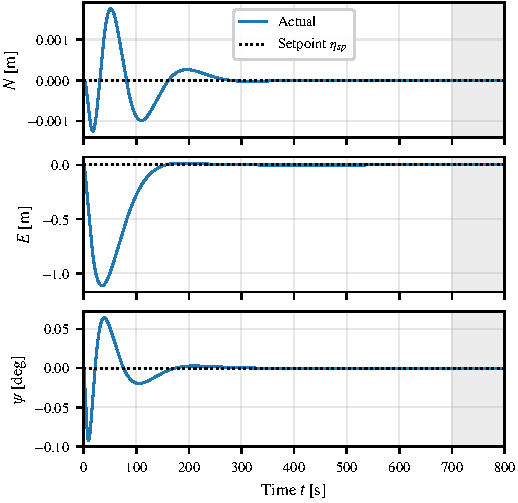
\includegraphics[width=\columnwidth]{sim1a_time.pdf}
  \caption{Simulation 1a: station keeping at $\eta_{sp}=[0,0,0]^\top$ in a $0.5$\,m/s current from east (no wind). North position, East position and heading. The shaded area is the last 100\,s used for steady-state metrics.}
  \label{fig:sim1a_time}
\end{figure}

\begin{figure}[!t]
  \centering
  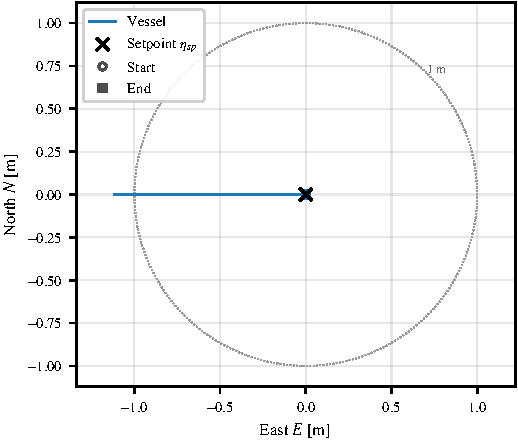
\includegraphics[width=\columnwidth]{sim1a_xy.pdf}
  \caption{Simulation 1a: $xy$-trajectory (North vs.\ East) in a $0.5$\,m/s current from east (no wind). Dotted circle(s) mark 1\,m from the setpoint.}
  \label{fig:sim1a_xy}
\end{figure}

\begin{figure}[!t]
  \centering
  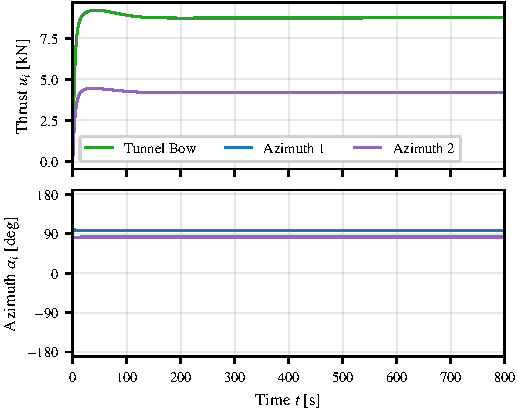
\includegraphics[width=\columnwidth]{sim1a_thrusters.pdf}
  \caption{Simulation 1a: thruster forces and azimuth angles in a $0.5$\,m/s current from east (no wind).}
  \label{fig:sim1a_thrusters}
\end{figure}

\begin{figure}[!t]
  \centering
  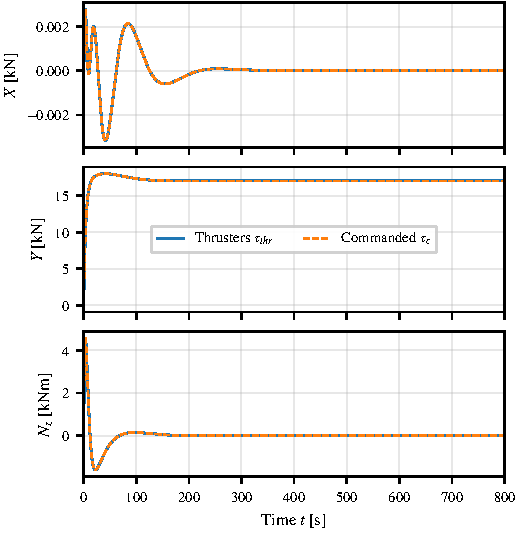
\includegraphics[width=\columnwidth]{sim1a_wrench.pdf}
  \caption{Simulation 1a: commanded and produced thruster wrench in a $0.5$\,m/s current from east (no wind).}
  \label{fig:sim1a_wrench}
\end{figure}

\begin{figure}[!t]
  \centering
  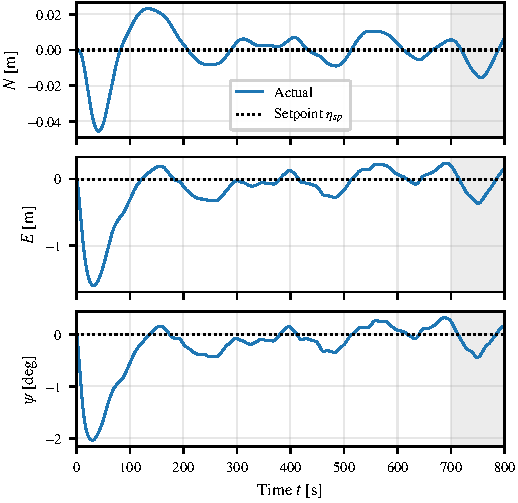
\includegraphics[width=\columnwidth]{sim1b_time.pdf}
  \caption{Simulation 1b: station keeping at $\eta_{sp}=[0,0,0]^\top$ in a $15$\,m/s mean wind from east with a slowly varying component ($\sigma=1$\,m/s, no current). North position, East position and heading. The shaded area is the last 100\,s used for steady-state metrics.}
  \label{fig:sim1b_time}
\end{figure}

\begin{figure}[!t]
  \centering
  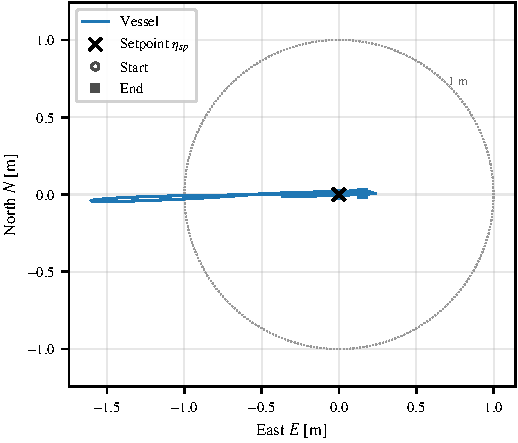
\includegraphics[width=\columnwidth]{sim1b_xy.pdf}
  \caption{Simulation 1b: $xy$-trajectory (North vs.\ East) in a $15$\,m/s mean wind from east with a slowly varying component ($\sigma=1$\,m/s, no current). Dotted circle(s) mark 1\,m from the setpoint.}
  \label{fig:sim1b_xy}
\end{figure}

\begin{figure}[!t]
  \centering
  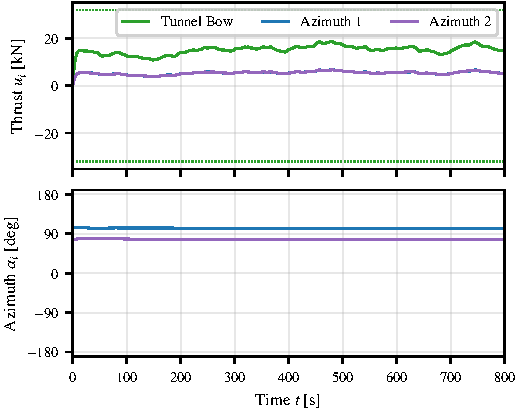
\includegraphics[width=\columnwidth]{sim1b_thrusters.pdf}
  \caption{Simulation 1b: thruster forces and azimuth angles in a $15$\,m/s mean wind from east with a slowly varying component ($\sigma=1$\,m/s, no current).}
  \label{fig:sim1b_thrusters}
\end{figure}

\begin{figure}[!t]
  \centering
  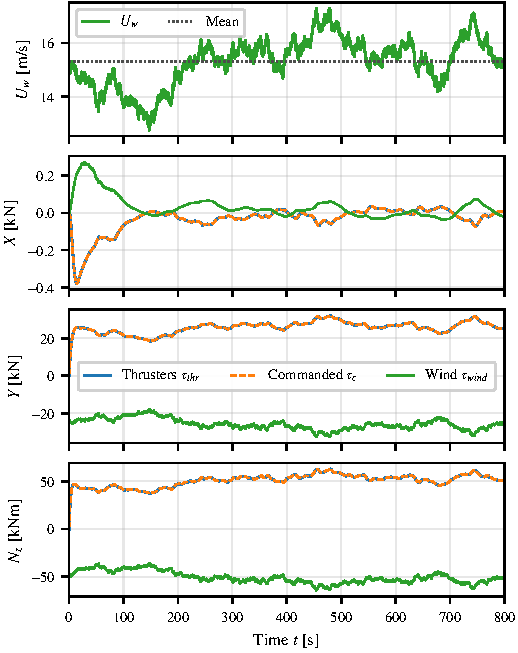
\includegraphics[width=\columnwidth]{sim1b_wrench.pdf}
  \caption{Simulation 1b: commanded and produced thruster wrench together with the wind load and wind speed in a $15$\,m/s mean wind from east with a slowly varying component ($\sigma=1$\,m/s, no current).}
  \label{fig:sim1b_wrench}
\end{figure}

% ======================================================================
% Simulation 2: rotating current
% ======================================================================
% Generated by resultspart1.py -- do not edit by hand
\begin{table}[!t]
\centering
\caption{Simulation 2: station keeping in a rotating current ($0.5$\,m/s, from north to from east over 300\,s). Metrics during the rotation, after it, and in the last 100\,s.}
\label{tab:sim2}
\footnotesize
\setlength{\tabcolsep}{3pt}
% shrink-to-fit: scaled down only if wider than the column/page
\sbox0{%
\begin{tabular}{lccc}
\toprule
Metric & $0$--$300$\,s & $300$--$900$\,s & Last $100$\,s \\
\midrule
Max.\ position error [m] & $0.34$ & $0.14$ & $0.00$ \\
\quad at time [s] & $151$ & $300$ & $800$ \\
Mean / RMS pos.\ error [m] & $0.25$ / $0.26$ & $0.01$ / $0.03$ & $0.00$ / $0.00$ \\
Max.\ heading error [deg] & $0.38$ & $0.39$ & $0.00$ \\
Mean heading error [deg] & $0.210$ & $0.036$ & $0.000$ \\
\midrule
Mean thr.\ $X$/$Y$/$N_z$ [kN, kNm] & $0.6$/$10.1$/$8.5$ & $0.0$/$17.1$/$0.0$ & $0.0$/$17.0$/$0.0$ \\
Mean thrust TB/A1/A2 [kN] & $5.5$/$2.4$/$2.4$ & $8.7$/$4.2$/$4.2$ & $8.7$/$4.2$/$4.2$ \\
Peak thrust TB/A1/A2 [kN] & $8.8$/$4.2$/$4.2$ & $8.8$/$4.2$/$4.2$ & $8.7$/$4.2$/$4.2$ \\
Saturated time [\%] & $0.0$ & $0.0$ & $0.0$ \\
\midrule
Settling after rot.\ ($<0.5$\,m) [s] & -- & $0.0$ & -- \\
\bottomrule
\end{tabular}}
\ifdim\wd0>\linewidth\resizebox{\linewidth}{!}{\usebox0}\else\usebox0\fi
\end{table}


\begin{figure}[!t]
  \centering
  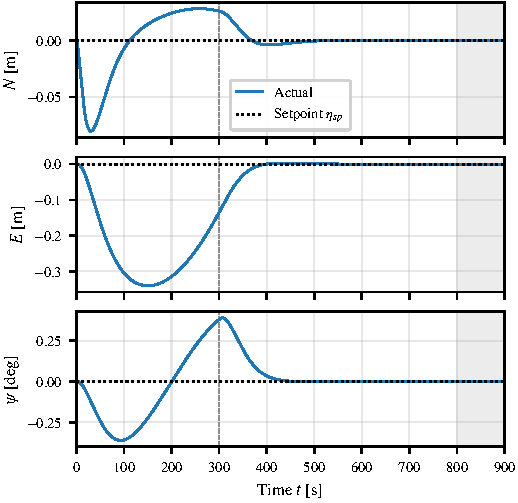
\includegraphics[width=\columnwidth]{sim2_time.pdf}
  \caption{Simulation 2: station keeping in a $0.5$\,m/s current whose direction rotates linearly from north to east over 300\,s (no wind). The dashed line marks the end of the current rotation; the shaded area is the steady-state window.}
  \label{fig:sim2_time}
\end{figure}

\begin{figure}[!t]
  \centering
  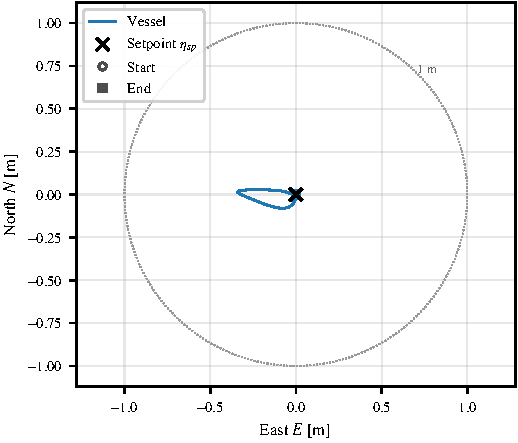
\includegraphics[width=\columnwidth]{sim2_xy.pdf}
  \caption{Simulation 2: $xy$-trajectory in a $0.5$\,m/s current whose direction rotates linearly from north to east over 300\,s (no wind). Dotted circle(s) mark 1\,m from the setpoint.}
  \label{fig:sim2_xy}
\end{figure}

\begin{figure}[!t]
  \centering
  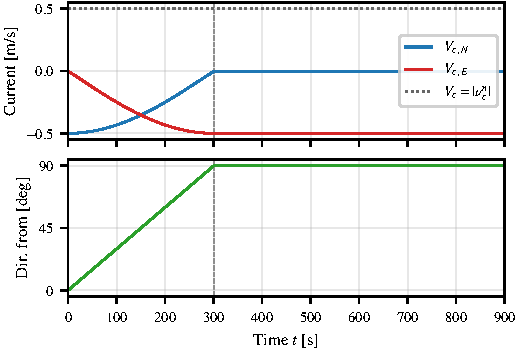
\includegraphics[width=\columnwidth]{sim2_current.pdf}
  \caption{Simulation 2: NED current components $V_{c,N}(t)$, $V_{c,E}(t)$ returned to the plant, and the direction the current comes from (0$^\circ$ = north, 90$^\circ$ = east).}
  \label{fig:sim2_current}
\end{figure}

\begin{figure}[!t]
  \centering
  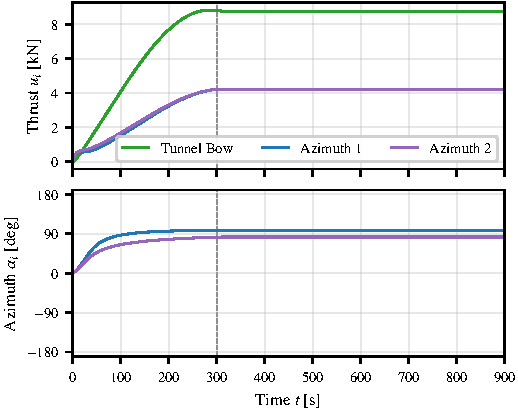
\includegraphics[width=\columnwidth]{sim2_thrusters.pdf}
  \caption{Simulation 2: thruster forces and azimuth angles during the rotating-current test.}
  \label{fig:sim2_thrusters}
\end{figure}

\begin{figure}[!t]
  \centering
  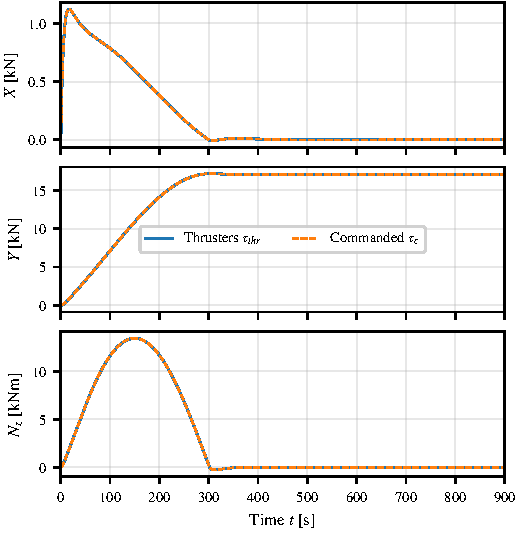
\includegraphics[width=\columnwidth]{sim2_wrench.pdf}
  \caption{Simulation 2: commanded and produced thruster wrench during the rotating-current test.}
  \label{fig:sim2_wrench}
\end{figure}

% ======================================================================
% Simulation 3: setpoint change with/without reference model
% ======================================================================
% Generated by resultspart1.py -- do not edit by hand
\begin{table}[!t]
\centering
\caption{Simulation 3: setpoint change from $[0,0,0]^\top$ to $[10,10,3\pi/2]^\top$ without environmental loads, with and without the reference model (identical controller and allocation). Final errors are means over the last 50\,s.}
\label{tab:sim3}
\footnotesize
\setlength{\tabcolsep}{3pt}
% shrink-to-fit: scaled down only if wider than the column/page
\sbox0{%
\begin{tabular}{lcc}
\toprule
Metric & With ref. & Without ref. \\
\midrule
Overshoot $N$ / $E$ [m] & $0.00$ / $0.00$ & $2.18$ / $2.30$ \\
Overshoot along path [m] & $0.00$ & $3.16$ \\
Heading overshoot [deg] & $11.47$ & $26.70$ \\
Rotation in wrong dir.\ [deg] & $0.00$ & $0.00$ \\
\midrule
Time to 90\,\% of translation [s] & $70.8$ & $25.5$ \\
Settling, pos.\ ($<0.5$\,m) [s] & $89.0$ & $130.5$ \\
Settling, head.\ ($<1^\circ$) [s] & $182.5$ & $182.6$ \\
Final position error [m] & $0.000$ & $0.000$ \\
Final heading error [deg] & $0.000$ & $0.000$ \\
\midrule
Max.\ dev.\ from straight line [m] & $0.20$ & $3.16$ \\
Path length (straight $14.14$) [m] & $14.20$ & $20.54$ \\
Max.\ speed / yaw rate [m/s, deg/s] & $0.27$ / $2.01$ & $0.65$ / $2.45$ \\
\midrule
Peak $|\tau_c|$ $X$/$Y$/$N_z$ [kN, kNm] & $9$/$15$/$528$ & $95$/$112$/$1355$ \\
Peak thrust TB/A1/A2 [kN] & $14.1$/$14.6$/$13.4$ & $21.9$/$75.3$/$67.6$ \\
Time saturated [\%] & $0.0$ & $0.0$ \\
$\int\sum_i|u_i|\,dt$ [MNs] & $1.70$ & $2.49$ \\
\bottomrule
\end{tabular}}
\ifdim\wd0>\linewidth\resizebox{\linewidth}{!}{\usebox0}\else\usebox0\fi
\end{table}


\begin{figure}[!t]
  \centering
  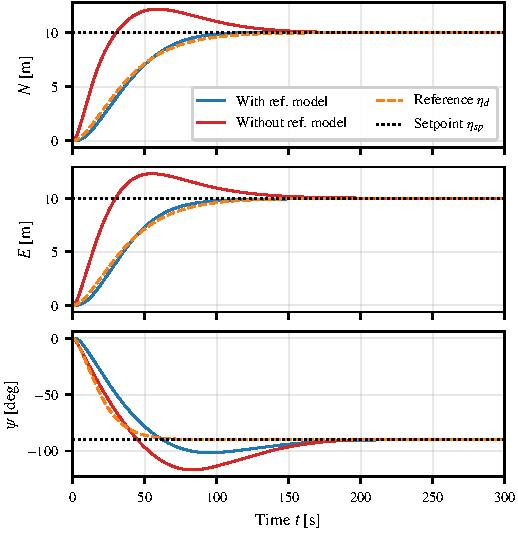
\includegraphics[width=\columnwidth]{sim3_time.pdf}
  \caption{Simulation 3: step from $\eta_0=[0,0,0]^\top$ to $\eta_{sp}=[10,10,3\pi/2]^\top$ ($3\pi/2 \equiv -\pi/2$), no environmental loads. Response with and without the reference model, the reference-model output $\eta_d$ and the setpoint.}
  \label{fig:sim3_time}
\end{figure}

\begin{figure}[!t]
  \centering
  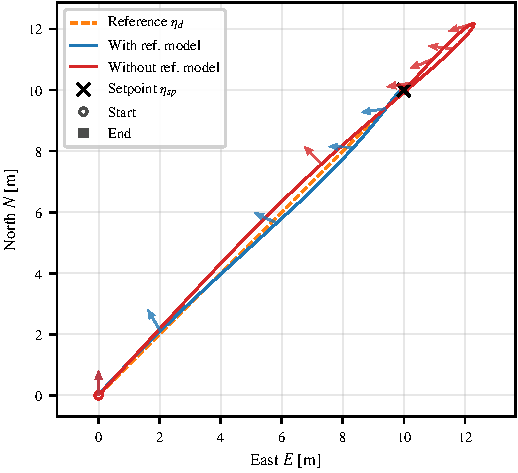
\includegraphics[width=\columnwidth]{sim3_xy.pdf}
  \caption{Simulation 3: $xy$-trajectories for the step from $\eta_0=[0,0,0]^\top$ to $\eta_{sp}=[10,10,3\pi/2]^\top$ ($3\pi/2 \equiv -\pi/2$), no environmental loads. Arrows show the vessel heading every 20\,s.}
  \label{fig:sim3_xy}
\end{figure}

\begin{figure}[!t]
  \centering
  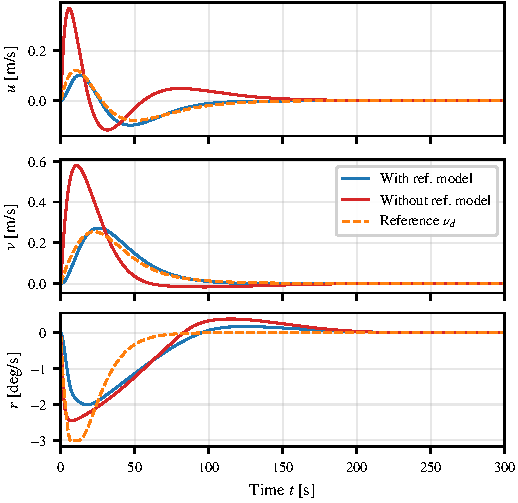
\includegraphics[width=\columnwidth]{sim3_velocities.pdf}
  \caption{Simulation 3: body-frame velocities $u$, $v$, $r$ with and without the reference model, together with the reference-model velocities $\nu_d$ (mapped to the body frame).}
  \label{fig:sim3_velocities}
\end{figure}

\begin{figure}[!t]
  \centering
  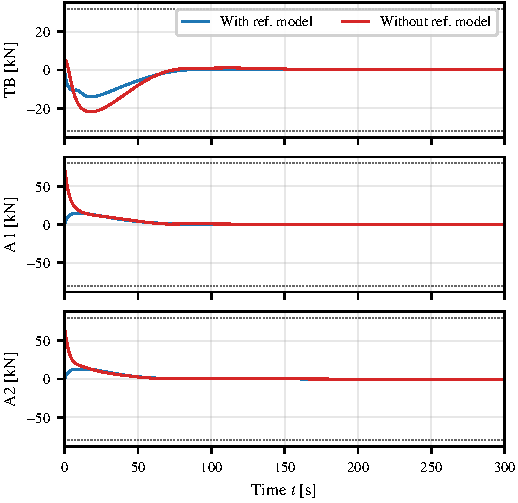
\includegraphics[width=\columnwidth]{sim3_thrusters.pdf}
  \caption{Simulation 3: thrust of the Tunnel Bow (TB) and Azimuth 1/2 (A1/A2) thrusters with and without the reference model (dotted: $\pm u_{\max}$).}
  \label{fig:sim3_thrusters}
\end{figure}

% ======================================================================
% Simulation 4: four-corner test
% ======================================================================
% Generated by resultspart1.py -- do not edit by hand
\begin{table*}[!t]
\centering
\caption{Simulation 4: four-corner test, metrics per leg (300\,s hold per setpoint, time measured from the setpoint switch). Settling bands: 0.5\,m and 1$^\circ$. OS = overshoot along the direction of travel; path dev.\ = max.\ distance from the straight line between setpoints; final errors are means over the last 50\,s of each leg; util.\ = peak thrust relative to $u_{\max}$ (worst thruster).}
\label{tab:sim4}
\footnotesize
\setlength{\tabcolsep}{3pt}
% shrink-to-fit: scaled down only if wider than the column/page
\sbox0{%
\begin{tabular}{llcccccccc}
\toprule
Leg & Setpoint $(N,E,\psi)$ & $t_{s,\mathrm{pos}}$ [s] & $t_{s,\psi}$ [s] & OS [m] & OS$_\psi$ [deg] & Path dev.\ [m] & $\bar e_{\mathrm{pos}}$ [m] & $\bar e_{\psi}$ [deg] & Util.\ [\%] \\
\midrule
$\eta_{0}\!\rightarrow\!\eta_{1}$ & $(50,\,0,\,0^\circ)$ & $170.1$ & $0.0$ & $0.00$ & -- & $0.00$ & $0.026$ & $0.000$ & $29$ \\
$\eta_{1}\!\rightarrow\!\eta_{2}$ & $(50,\,-50,\,0^\circ)$ & $137.4$ & $0.0$ & $0.04$ & -- & $0.04$ & $0.011$ & $0.013$ & $87$ \\
$\eta_{2}\!\rightarrow\!\eta_{3}$ & $(50,\,-50,\,-45^\circ)$ & $0.0$ & $147.4$ & -- & $3.99$ & $0.03$ & $0.000$ & $0.016$ & $25$ \\
$\eta_{3}\!\rightarrow\!\eta_{4}$ & $(0,\,-50,\,-45^\circ)$ & $155.2$ & $0.0$ & $0.00$ & -- & $0.55$ & $0.020$ & $0.009$ & $57$ \\
$\eta_{4}\!\rightarrow\!\eta_{5}$ & $(0,\,0,\,0^\circ)$ & $138.2$ & $146.7$ & $0.04$ & $3.47$ & $0.50$ & $0.011$ & $0.004$ & $87$ \\
\bottomrule
\end{tabular}}
\ifdim\wd0>\linewidth\resizebox{\linewidth}{!}{\usebox0}\else\usebox0\fi
\end{table*}


\begin{figure*}[!t]
  \centering
  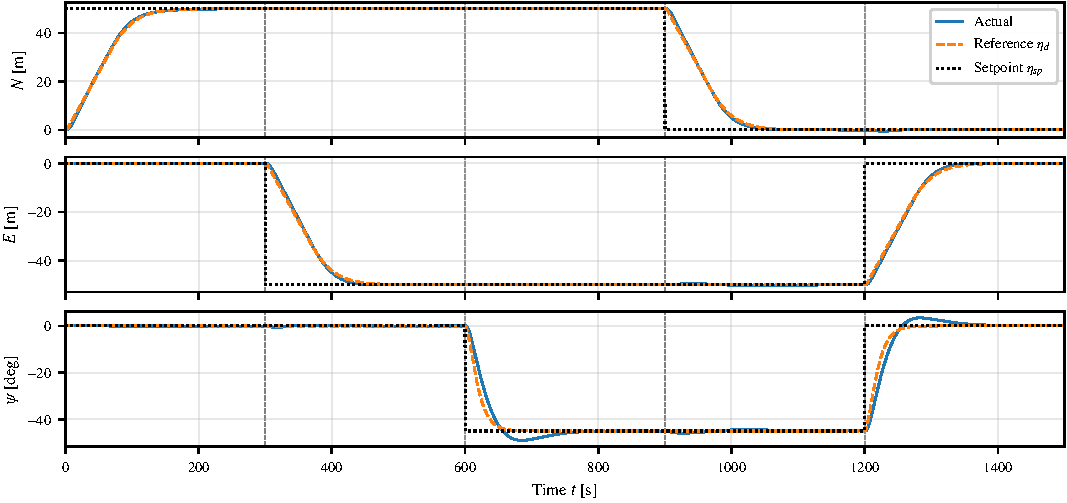
\includegraphics[width=\textwidth]{sim4_time.pdf}
  \caption{Simulation 4: four-corner test without environmental loads. North, East and heading with the reference-model output $\eta_d$ and the setpoint. Setpoints switch every 300\,s (dashed lines).}
  \label{fig:sim4_time}
\end{figure*}

\begin{figure}[!t]
  \centering
  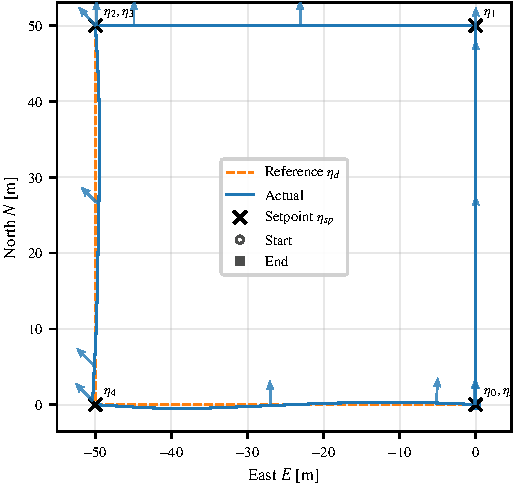
\includegraphics[width=\columnwidth]{sim4_xy.pdf}
  \caption{Simulation 4: $xy$-trajectory of the four-corner test with the reference path. Arrows show the vessel heading every 50\,s.}
  \label{fig:sim4_xy}
\end{figure}

\begin{figure*}[!t]
  \centering
  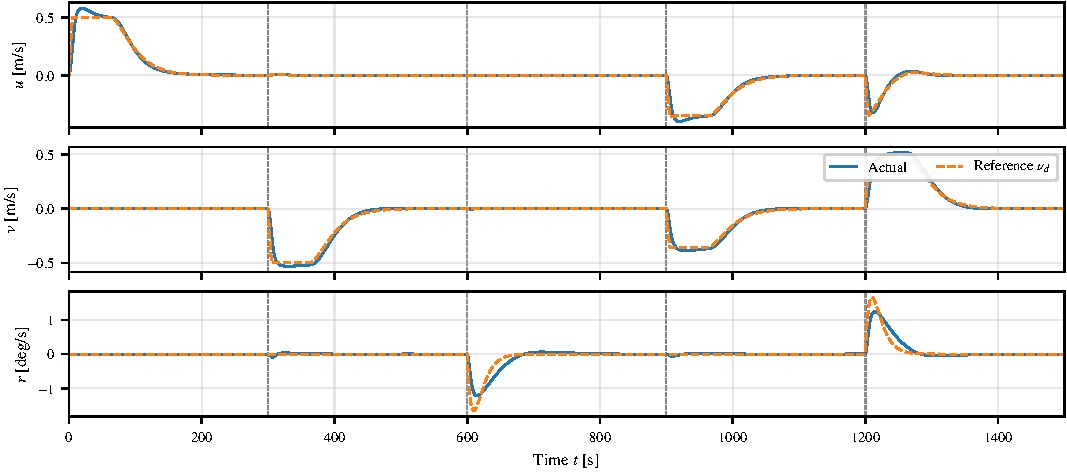
\includegraphics[width=\textwidth]{sim4_velocities.pdf}
  \caption{Simulation 4: body-frame velocities $u$, $v$, $r$ and the reference-model velocities $\nu_d$ (mapped to the body frame).}
  \label{fig:sim4_velocities}
\end{figure*}

\begin{figure*}[!t]
  \centering
  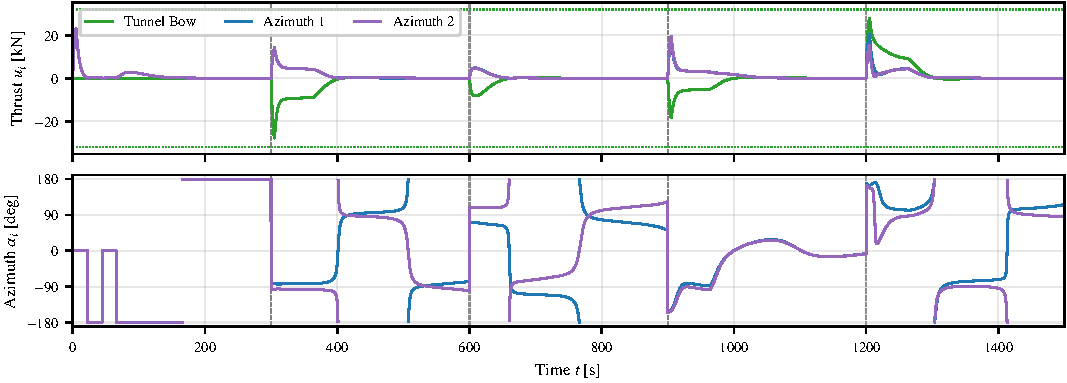
\includegraphics[width=\textwidth]{sim4_thrusters.pdf}
  \caption{Simulation 4: thruster forces (dotted: $\pm u_{\max}$ of the Tunnel Bow thruster) and azimuth angles during the four-corner test.}
  \label{fig:sim4_thrusters}
\end{figure*}
